% concatenated from ms.tex
% Template for Electronic Journal of Graph Theory and Applications
% This file must be in the same folder as EJGTAart.sty and EJGTAhead.jpg

\documentclass[12pt]{elsarticle}
\usepackage[left=1in,right=1in, top=1.2in,bottom=1.2in]{geometry}
%\usepackage{EJGTAart}
\usepackage{times}
\usepackage{amssymb,amsthm,latexsym,amsmath,epsfig,pgf,tikz,multirow}
\usepackage{lineno,booktabs}
\usepackage{pdflscape}
\usetikzlibrary{shapes.geometric,calc}
\usetikzlibrary{arrows.meta}
\usepackage{hyperref}
\hypersetup{
	colorlinks=true,
	linkcolor=blue,
	filecolor=magenta,      
	urlcolor=cyan,
	pdftitle={Overleaf Example},
	pdfpagemode=FullScreen,
}


% Put new theorem or any other settings for your document here
\newtheorem{theorem}{Theorem}[section]
\newtheorem*{theorem A}{Theorem A}
\newtheorem*{theorem B}{N\"olker's Theorem}
\newtheorem{lemma}{Lemma}[section]
\newtheorem{proposition}{Proposition}[section]
\newtheorem{observation}{Observation}
\newtheorem{corollary}{Corollary}[section]
\newtheorem{problem}{Problem}
\newtheorem*{question}{Question}
\newtheorem {conjecture}{Conjecture}
\theoremstyle{remark}
\newtheorem{remark}{Remark}[section]
\theoremstyle{remark}
\newtheorem{remarks}{Remarks}
\theoremstyle{definition}
\newtheorem{definition}{Definition}
\begin{document}

\begin{frontmatter}
% Write your paper title here
%% use optional labels to link authors explicitly to addresses. The label may be more than one, use comma to separate

%\author[label1,label]{Edy Tri Baskoro${}^1$}
\title{Node-Kayles on Trees}
\author[label1]{Nuttanon Songsuwan}
%\author[label2]{Joe Ryan}
%\author[label3]{Kiki A. Sugeng}

\address[label1]{\small Faculty of Science at Sriracha, Kasetsart University, Sriracha Campus, Thailand

\vspace*{2.5ex} 
{\normalfont nuttanon.son@ku.th}}
%\address[label2]{School of Electrical Engineering and Computer Science,
%The University of Newcatle, Australia}
%\address[label3]{Departments of Mathematics,
%University of Indonesia,
%Depok - Indonesia

%\vspace*{2.5ex} 
% {\normalfont ebaskoro@math.itb.ac.id, joe.ryan@newcastle.edu.au, kiki@sci.ui.ac.id}
% }

\begin{abstract}
Node-Kayles is a well-known impartial combinatorial game played on graphs, where players alternately select a vertex and remove it along with its neighbors. By the Sprague–Grundy theorem, every position of an impartial game corresponds to a non-negative integer called its Grundy value. In this paper, we investigate the Grundy value sequences of $n$-regular trees as well as graphs formed by joining two $n$-regular trees with a path of length $k$. We derive explicit formulas and recursive relations for the associated Grundy value sequences. Furthermore, we prove that these sequences are eventually periodic and determine both their preperiod lengths and their periods.

\let\thefootnote\relax\footnotetext{Received: xx xxxxx 20xx,\quad
  Accepted: xx xxxxx 20xx.\\[3ex]
  }
  
\end{abstract}

\begin{keyword}
% Separate keyword by \sep
Combinatorial game \sep Grundy value \sep Impartial game  \sep Node-Kayles

% Write the classification number
Mathematics Subject Classification : 05C57 \sep 91A05 \sep 91A46

\end{keyword}

\end{frontmatter}

%% Main text
\section{Introduction}
Impartial combinatorial games form a central object of study in combinatorial game theory. They are two-player, perfect-information, finite games without chance, in which the set of legal moves from any position is the same for both players and the winner is determined under the normal-play convention by making the last move \cite{brown2020nimber, conway2000numbers, berlekamp2001winning}. Classic examples include Nim, subtraction and taking-and-breaking games, and various graph-based games such as Node-Kayles \cite{brown2020nimber, berlekamp2001winning,albert2019lessons}. The unifying mathematical framework for such games is provided by the Sprague–Grundy theorem, developed independently by Sprague \cite{sprague1935mathematische} in 1936 and Grundy \cite{grundy1939mathematics} in 1939 and popularized in the work of Conway and of Berlekamp, Conway, and Guy \cite{conway2000numbers, berlekamp2001winning}.

The Sprague–Grundy theorem asserts that every impartial game position $G$ is equivalent, under normal play, to a single Nim heap of some nonnegative integer size, called its Grundy value or Grundy value $\mathcal{G}(G)$. The terminal position has Grundy value $0$, and and a position has Grundy value
$0$ if and only if it is a $\mathcal{P}$-position, i.e., a second-player win with perfect play. The Grundy value of position is defined recursively by the minimum excluded value (mex) rule: if
$O(G)$ is the set of options (positions reachable in one move) from$G$ and $S = \left\{\mathcal{G}(H) : H \in O(G)\right\}$ is the set of Grundy values of these options, then
\begin{equation*}
	\mathcal{G}(G) = \mathrm{mex}(S),
\end{equation*}
where $\mathrm{mex}(S)$ is the least nonnegative integer not in $S$ \cite{brown2020nimber, bodlaender2002kayles}. This maximum-excluded (mex) rule gives a purely combinatorial procedure for computing Grundy values from the game graph.

A second pillar of Sprague–Grundy theory is the behavior of impartial games under disjoint sum. When a game decomposes into independent components $G = G_1 + G_2 + \dots + G_k$ (each move affects exactly one component), the Grundy value of $G$ is the nim-sum (bitwise XOR) of the Grundy values of its components:
\begin{equation*}
	\mathcal{G}(G) = \bigoplus_{i=1}^{k}\mathcal{G}(G_i) = \mathcal{G}(G_1) \oplus \mathcal{G}(G_2) \oplus \dots \oplus \mathcal{G}(G_k).
\end{equation*}
Here $\oplus$ denotes binary addition without carry \cite{brown2020nimber,albert2019lessons,bodlaender2002kayles}. This rule reduces the analysis of complex disjoint unions to that of their connected components and makes Grundy values a powerful algebraic invariant of impartial games.

Node-Kayles, also known as the domination game in some graph-theoretic contexts \cite{duchene2009combinatorial}, is a canonical impartial game played on a simple graph $G = (V,E)$. In the normal version of Node-Kayles, players alternate choosing a vertex $v \in V$; a move removes $v$, all its neighbors $N_{G}(v)$, and all incident edges from the graph, leaving the induced subgraph $G_{v} = G \backslash N_{G}[v]$, where $N_{G}[v] = \{v\} \cup N_{G}(v)$ is the closed neighborhood of $v$. The player who first has no legal move loses. The game is impartial because both players have the same set of moves from any given position, and it is finite under normal play. Node-Kayles has been studied from both complexity-theoretic and structural perspectives: deciding the winner on general graphs is PSPACE-complete \cite{bodlaender2015exact,fleischer2004kayles}, while polynomial-time algorithms exist for various restricted graph classes such as graphs of bounded asteroidal number, cocomparability graphs, cographs, and others \cite{guignard2009compound,bodlaender2002kayles}.

From the Sprague–Grundy viewpoint, each simple graph $G$ has an associated Grundy value $\mathcal{G}(G)$, defined recursively by
\begin{equation*}
	\mathcal{G}(G) = \mathrm{mex}\{\mathcal{G}(G_{v}): v \in V(G)\},
\end{equation*}
where $\mathcal{G}(\emptyset) = 0$, and for a disjoint union $G = H \cup K$,
\begin{equation*}
	\mathcal{G}(G) = \mathcal{G}(H) \oplus \mathcal{G}(K).
\end{equation*}

To illustrate these definitions, consider Node-Kayles on some simple graphs and compute their respective Grundy values. Let $K_n$ denote a complete graph with $n$ vertices. Since the closed neighborhood of complete graph is $V(K_n)$ itself, so the only move leaves the empty graph. Thus
\begin{equation*}
	\mathcal{G}(K_n) = \mathrm{mex}\{\mathcal{G}(\emptyset)\} = \mathrm{mex}\{0\} = 1.
\end{equation*}
for every integer $n$. Let $P_n$ denote a path on $n$ vertices. For $P_1$, the only vertex $v$ has closed neighborhood $N[v] = V(P_1)$, so the only move also leaves the empty graph. Thus
\begin{equation*}
	\mathcal{G}(P_1) = \mathrm{mex}\{\mathcal{G}(\emptyset)\} = \mathrm{mex}\{0\} = 1.
\end{equation*}
For $P_2$, either endpoint has closed neighborhood equal to all of $P_2$, so any move again leaves the empty graph, and
\begin{equation*}
	\mathcal{G}(P_2) = \mathrm{mex}\{\mathcal{G}(\emptyset)\} = 1.
\end{equation*}
For $P_3$ with vertices $v_1,v_2$ and $v_3$, playing at $v_2$ removes all vertices and leaves empty graph (Grundy value of $0$), while playing at $v_1$ or $v_3$ leaves a single isolated vertex $P_1$ (Grundy value of $1$). Hence the set of option Grundy values from $P_3$ is $\{0,1\}$, and
\begin{equation*}
	\mathcal{G}(P_2) = \mathrm{mex}\{0,1\} = 2.
\end{equation*}
If $G$ is a graph in Figure \ref{fig:ex1}, then as seen in Figure \ref{fig:ex2}, the induced subgraphs $G_{v_1}$ and $G_{v_2}$ are isomorphic to $P_1 \cup K_3$, while the induced subgraph $G_{v_4}$ and $G_{v_5}$ are isomorphic to $P_1 \cup P_1$ and $G_{v_3}$ and $G_{v_6}$ are isomorphic to $P_1$ and $P_3$, respectively.
\begin{figure}[!ht]
	\centering
	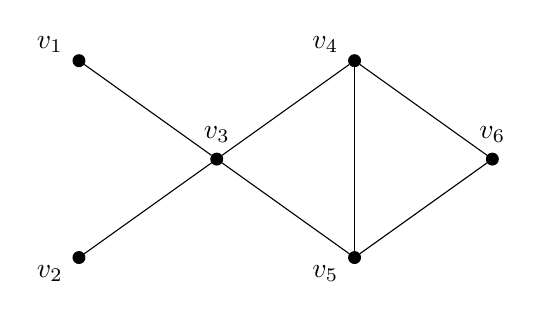
\begin{tikzpicture}
		\tikzset{enclosed/.style={draw, circle, inner sep=0pt, minimum size=.15cm, fill=black}}
		
		\node[enclosed, label={left, yshift=.2cm: $v_1$}] (1) at (0.75,3.25) {};
		\node[enclosed, label={above, yshift=0cm: $v_3$}] (3) at (2.5,2) {};
		\node[enclosed, label={left, yshift=-.2cm: $v_2$}] (2) at (0.75,0.75) {};
		\node[enclosed, label={left, yshift=.2cm: $v_4$}] (4) at (4.25,3.25) {};
		\node[enclosed, label={above, yshift=0cm: $v_6$}] (6) at (6,2) {};
		\node[enclosed, label={left, yshift=-.2cm: $v_5$}] (5) at (4.25,0.75) {};
		
		\draw (1) -- (3) node[midway, sloped, above] (edge1) {};
		\draw (2) -- (3) node[midway, right] (edge2) {};
		\draw (3) -- (4) node[midway, sloped, above] (edge3) {};
		\draw (3) -- (5) node[midway, sloped, above] (edge4) {};
		\draw (5) -- (4) node[midway, sloped, above] (edge5) {};
		\draw (6) -- (4) node[midway, sloped, above] (edge6) {};
		\draw (6) -- (5) node[midway, sloped, above] (edge7) {};
	\end{tikzpicture}
	\caption{A simple graph $G$ \label{fig:ex1}}
\end{figure}
\begin{figure}[!ht]
	\centering
	\begin{tikzpicture}
		\tikzset{enclosed/.style={draw, circle, inner sep=0pt, minimum size=.15cm, fill=black}}
		\node[] (1) at (1.25,0) {$G_{v_1}$};
		\node[] (2) at (4,0) {$G_{v_2}$};
		\node[] (3) at (6.75,0) {$G_{v_3}$};
		\node[] (4) at (9.5,0) {$G_{v_4}$};
		\node[] (5) at (12.25,0) {$G_{v_5}$};
		\node[] (6) at (15,0) {$G_{v_6}$};
		
		\node[enclosed, label={left, yshift=.2cm: $v_2$}] (12) at (0.5,1.5) {};
		\node[enclosed, label={above, yshift=.2cm: $v_4$}] (14) at (1,2.25) {};
		\node[enclosed, label={left, yshift=.2cm: $v_5$}] (15) at (1,0.75) {};
		\node[enclosed, label={above, yshift=.2cm: $v_6$}] (16) at (2,1.5) {};
		\draw (14) -- (15);
		\draw (14) -- (16);
		\draw (16) -- (15);
		
		\node[enclosed, label={left, yshift=.2cm: $v_1$}] (21) at (3.25,1.5) {};
		\node[enclosed, label={above, yshift=.2cm: $v_4$}] (24) at (3.75,2.25) {};
		\node[enclosed, label={left, yshift=.2cm: $v_5$}] (25) at (3.75,0.75) {};
		\node[enclosed, label={above, yshift=.2cm: $v_6$}] (26) at (4.75,1.5) {};
		\draw (24) -- (25);
		\draw (24) -- (26);
		\draw (26) -- (25);
		
		\node[enclosed, label={left, yshift=.2cm: $v_6$}] (36) at (6.75,1.5) {};
		
		\node[enclosed, label={left, yshift=.2cm: $v_1$}] (41) at (9.5,2.25) {};
		\node[enclosed, label={left, yshift=.2cm: $v_2$}] (42) at (9.5,0.75) {};
		
		\node[enclosed, label={left, yshift=.2cm: $v_1$}] (51) at (12.25,2.25) {};
		\node[enclosed, label={left, yshift=.2cm: $v_2$}] (52) at (12.25,0.75) {};
		
		\node[enclosed, label={above, yshift=.2cm: $v_1$}] (61) at (14.5,2.25) {};
		\node[enclosed, label={left, yshift=.2cm: $v_2$}] (62) at (14.5,0.75) {};
		\node[enclosed, label={above, yshift=.2cm: $v_3$}] (63) at (15.5,1.5) {};
		\draw (61) -- (63);
		\draw (62) -- (63);
	\end{tikzpicture}
	\caption{The induced subgraphs $G_{v_1}, G_{v_2}, G_{v_3}, G_{v_4}, G_{v_5}$ and $G_{v_6}$ \label{fig:ex2}}
\end{figure}

\noindent Therefore,
\begin{align*}
	\mathcal{G}(G) &= \mathrm{mex}\{\mathcal{G}(G_{v_i}): i = 1,2,3,4,5,6\}\\
	&= \mathrm{mex}\{\mathcal{G}(P_1 \cup K_3), \mathcal{G}(P_1 \cup P_1), \mathcal{G}(P_1), \mathcal{G}(P_3)\}\\
	&= \mathrm{mex}\{\mathcal{G}(P_1) \oplus \mathcal{G}(K_3), \mathcal{G}(P_1) \oplus \mathcal{G}(P_1), \mathcal{G}(P_1), \mathcal{G}(P_3)\}\\
	&= \mathrm{mex}\{1 \oplus 1, 1 \oplus 1, 1, 2\}\\
	&= \mathrm{mex}\{0, 1, 2\} = 3.
\end{align*}
This simple example shows how the $\mathrm{mex}$ rule and disjoint-union rule ($\oplus$) combine to yield Grundy values in practice.

Node-Kayles is a generalization of Kayles \cite{berlekamp2003winning}, independently introduced by Dudeney \cite{dudeney2002canterbury} and Loyd \cite{loyd1976sam}. Playing Node-Kayles on a path is equivalent to a particulat \textit{Take-and-Break} game introduced by Dawson \cite{dawson1935caissa}, and now known as \textit{Dawson's chess}, which corresponds to the octal game $.137$ (see \cite{berlekamp2003winning,conway2000numbers,flammenkamp2000sprague} for more details). This consists of removing $1,2$ or $3$ counters with certain options to shorten or split the heap, see Table \ref{octal}. 
\begin{table}[]\label{octal}
	\centering
	\begin{tabular}{|c|c|l|}
		\hline
		Octal digit & \begin{tabular}[c]{@{}c@{}}Binary\\ (bits)\end{tabular} & \multicolumn{1}{c|}{Allowed actions for a removal of $i$ counters}                                                                                                      \\ \hline
		0           & 000                                                     & No legal move of size $i$ (the player cannot remove exactly $i$ counters).                                                                                              \\ \hline
		1           & 001                                                     & \begin{tabular}[c]{@{}l@{}}Take-all only. The player may remove exactly $i$ counters and \\ the heap becomes empty.\end{tabular}                                        \\ \hline
		2           & 010                                                     & \begin{tabular}[c]{@{}l@{}}Reduce only. The player may remove exactly $i$ counters and leave \\ a single smaller heap (the remainder is kept as one heap).\end{tabular} \\ \hline
		3           & 011                                                     & \begin{tabular}[c]{@{}l@{}}Take-all or Reduce. \\ Both options are permitted for a removal of $i$ counters.\end{tabular}                                                \\ \hline
		4           & 100                                                     & \begin{tabular}[c]{@{}l@{}}Split only. After removing $i$ counters the remainder must be divided \\ into two non‑empty heaps.\end{tabular}                              \\ \hline
		5           & 101                                                     & Take‑all or Split.                                                                                                                                                      \\ \hline
		6           & 110                                                     & Reduce or Split.                                                                                                                                                        \\ \hline
		7           & 111                                                     & Take‑all, Reduce, or Split                                                                                                                                              \\ \hline
	\end{tabular}
	\caption{Interpretation of Octal game code}
\end{table}
In that
sense, $.137$ means: one single vertex can only be removed if it has no outgoing edges (anymore). Two vertices can only be removed if they form one connected component or if after their removal the remaining part of that connected component is still connected. For three vertices we have more possibilities. We are allowed to remove them if the remaining vertices are left in at most two connected components.


\begin{theorem}
	The Grundy value sequence ($\mathcal{G}(P_n):n \in \mathbb{N}$) is eventually periodic sequence with preperiod of length 51 and period 34.
\end{theorem}
The periodic part of the sequence for $n \equiv 0,1,2 \dots ,33 (\mod 34)$ are
\begin{equation*}
	8,1,1,2,0,3,1,1,0,3,3,2,2,4,4,5,5,9,3,3,0,1,1,3,0,2,1,1,0,4,5,3,7,4.
\end{equation*}
The Grundy value sequence ($\mathcal{G}(P_n): 0\le n \le 441$) can be seen in Table \ref{Pk} and coincides with OEIS sequence \href{https://oeis.org/A002187}{A002187}. This analysis has been extended to a wide range of Node-Kayles graph families, including powers and variants of paths, lattice graphs, prism graphs, chained and linked cliques, linked cycles and diamonds, hypercubes, and generalized Petersen graphs, often yielding explicit or recursive descriptions of their Grundy value sequences \cite{brown2020nimber, fleischer2004kayles, guignard2009compound}.

In this work we focus on the Grundy value sequences of Node-Kayles on rooted trees and on new graph operations that systematically build larger graphs from rooted components. We introduce a rooted grafting operation that joins two rooted graphs by a path connecting their distinguished roots, producing a new graph. Using the Sprague-Grundy framework, we derive recursive descriptions of the Grundy value of these rooted graftings in terms of the Grundy values of the constituent rooted trees and the length of the connecting path. We then investigate the resulting Grundy value sequences for infinite families of rooted trees $\left(T_{\{n\}}: n \in \mathbb{N}\right)$ and $\left(T_{\{n,m\}}: n,m \in \mathbb{N}\right)$ in Section \ref{sec2}. We then present Grundy value sequence on the rooted graftings $\left(T_{\{m\}} \stackrel{k}{\cdot - \cdot} T_{\{n\}} : k,n,m \in \mathbb{N}\right)$ through the computation, and we prove that all of these sequences are eventually periodic in Section \ref{sec3}. Our results thus provide new structured examples where periodicity of Grundy value sequences can be established rigorously, extending the catalog of Node-Kayles graph families with known Grundy value behavior and contributing evidence and techniques relevant to periodicity questions in octal and graph-based impartial games.

\section{Node-Kayles on rooted tree}\label{sec2}
In this section, we investigate the Grundy value associated with Node-Kayles played on $n$-regular trees.
\begin{definition}
	The $n$-regular tree $T_{\{a_i\}_{i=0}^{n}}$ is a rooted tree of depth $n+1$, where each vertex at level $i$ (with the root at level $0$) has exactly $a_{i}$ children, for $i = 0,1,\dots, n$. The branching factor at each level is determined by the sequence $\{a_0,a_1,\dots,a_n\}$.
\end{definition}

\begin{theorem}
The Grundy value sequence $\left(\mathcal{G}\left(T_{\{n\}}\right) : n \in \mathbb{N}\right)$ are given by the following:
\begin{equation*}
	\mathcal{G}\left(T_{\{n\}}\right) = \begin{cases}
		1,	\quad \text{if $n$ is odd};\\
		2,	\quad \text{if $n$ is even}
	\end{cases}
\end{equation*}
for all $n \in \mathbb{N}$
\end{theorem}
\begin{proof}
	By definition,
	\begin{equation*}
		\mathcal{G}\left(T_{\{n\}}\right) = \mathrm{mex}\left\{\mathcal{G}\left(\emptyset\right), \bigoplus_{i=1}^{n-1}\mathcal{G}\left(\cdot\right)\right\}
	\end{equation*}
	with $\mathcal{G}\left(\emptyset\right) = 0$ and $\mathcal{G}\left(\cdot\right) = 1$. By the definition of disjoint union,
	\begin{equation*}
		\bigoplus_{i=1}^{n-1}\mathcal{G}\left(\cdot\right) = \begin{cases}
			0,	\quad \text{if $n$ is odd};\\
			1,	\quad \text{if $n$ is even}.
		\end{cases}
	\end{equation*}
	Therefore, 
	\begin{equation*}
		\mathcal{G}\left(T_{\{n\}}\right) = \begin{cases}
			1,	\quad \text{if $n$ is odd};\\
			2,	\quad \text{if $n$ is even.}
		\end{cases}
	\end{equation*}
\end{proof}
\begin{theorem}\label{Tnm}
	The Grundy value sequence $\left( \mathcal{G}\left(T_{\{n,m\}}\right) : n,m \in \mathbb{N} \right)$ are given by the following:
	\begin{equation*}
		\mathcal{G}\left(T_{\{n,m\}}\right) = \begin{cases}
			1,	\quad \text{if $m$ is even};\\
			2,	\quad \text{if $n,m$ are odd};\\
			3,	\quad \text{if $n$ is even and $m$ is odd}
		\end{cases}
	\end{equation*}
	for all $n \in \mathbb{N}$
\end{theorem}
\begin{proof}
	The move of the first player is consist of 3 action
	\begin{itemize}
		\item play at the root: $\bigoplus_{i=1}^{n\cdot m}\mathcal{G}\left(\cdot\right)$
		\item play at the first level: $\bigoplus_{i=1}^{n-1}\mathcal{G}\left(T_{\{m\}}\right)$
		\item play at the second level: $\mathcal{G}\left(T_{\{n-1,m\}}\right) \oplus \bigoplus_{i=1}^{m-1}\mathcal{G}\left(\cdot\right)$
	\end{itemize}
	By the definition,
	\begin{equation*}
		\mathcal{G}\left(T_{\{n,m\}}\right) = \mathrm{mex}\left\{\bigoplus_{i=1}^{n\cdot m}\mathcal{G}\left(\cdot\right), \bigoplus_{i=1}^{n-1}\mathcal{G}\left(T_{\{m\}}\right), \mathcal{G}\left(T_{\{n-1,m\}}\right) \oplus \bigoplus_{i=1}^{m-1}\mathcal{G}\left(\cdot\right)\right\}
	\end{equation*}
	Suppose $m$ is even. It is easy to see that $\mathcal{G}\left(T_{\{1,m\}}\right) = \mathcal{G}\left(T_{\{m+1\}}\right) =  1$, $\bigoplus_{i=1}^{n\cdot m}\mathcal{G}\left(\cdot\right) = 0$ and
	\begin{equation*}
		\bigoplus_{i=1}^{n-1}\mathcal{G}\left(T_{\{m\}}\right) = \begin{cases}
			0,	\quad \text{if $n$ is odd};\\
			2,	\quad \text{if $n$ is even}.
		\end{cases}
	\end{equation*} By using induction,
	\begin{align*}
		\mathcal{G}\left(T_{\{n,m\}}\right) &= \mathrm{mex}\left\{\bigoplus_{i=1}^{n\cdot m}\mathcal{G}\left(\cdot\right), \bigoplus_{i=1}^{n-1}\mathcal{G}\left(T_{\{m\}}\right), \mathcal{G}\left(T_{\{n-1,m\}}\right) \oplus \bigoplus_{i=1}^{m-1}\mathcal{G}\left(\cdot\right)\right\}\\
		&= \mathrm{mex}\left\{0, (0 \text{ or } 2), \mathcal{G}\left(T_{\{n-1,m\}}\right) \oplus  1\right\}\\
		&= \mathrm{mex}\left\{0, (0 \text{ or } 2), 1 \oplus  1\right\}\\
		&= \mathrm{mex}\left\{0, (0 \text{ or } 2)\right\}\\
		&= 1.
	\end{align*}
	If $m$ is odd, then $\mathcal{G}\left(T_{\{1,m\}}\right) = \mathcal{G}\left(T_{\{m+1\}}\right) =  2$,
	\begin{equation*}
			\bigoplus_{i=1}^{n\cdot m}\mathcal{G}\left(\cdot\right) = \begin{cases}
				0,	\quad \text{if $n$ is even};\\
				1,	\quad \text{if $n$ is odd}
			\end{cases}
	\end{equation*}
	and
	\begin{equation*}
		\bigoplus_{i=1}^{n-1}\mathcal{G}\left(T_{\{m\}}\right) = \begin{cases}
			0,	\quad \text{if $n$ is odd};\\
			1,	\quad \text{if $n$ is even}.
		\end{cases}
	\end{equation*}
	We left to show that $\mathcal{G}\left(T_{\{2,m\}}\right) =  3$. The Grundy value of $\mathcal{G}\left(T_{\{2,m\}}\right)$ is
	\begin{align*}
		\mathcal{G}\left(T_{\{2,m\}}\right) &= \mathrm{mex}\left\{\bigoplus_{i=1}^{2 m}\mathcal{G}\left(\cdot\right), \mathcal{G}\left(T_{\{m\}}\right), \mathcal{G}\left(T_{\{1,m\}}\right) \oplus \bigoplus_{i=1}^{m-1}\mathcal{G}\left(\cdot\right)\right\}\\
		&= \mathrm{mex}\left\{0, 1, 2 \oplus 0\right\}\\
		&= \mathrm{mex}\left\{0, 1, 2 \right\}\\
		&= 3
	\end{align*}
	We are ready to finish our proof by strong induction. Assume that for some integer $n \ge 2$, 
	\begin{equation*}
		\mathcal{G}\left(T_{\{i,m\}}\right) = \begin{cases}
			2,	\quad \text{if $i$ are odd};\\
			3,	\quad \text{if $i$ is even}
		\end{cases}
	\end{equation*}
	for all integers $1 \le i < n$. If $n$ is odd, we get
	\begin{align*}
		\mathcal{G}\left(T_{\{n,m\}}\right) &= \mathrm{mex}\left\{\bigoplus_{i=1}^{n\cdot m}\mathcal{G}\left(\cdot\right), \bigoplus_{i=1}^{n-1}\mathcal{G}\left(T_{\{m\}}\right), \mathcal{G}\left(T_{\{n-1,m\}}\right) \oplus \bigoplus_{i=1}^{m-1}\mathcal{G}\left(\cdot\right)\right\}\\
		&= \mathrm{mex}\left\{1,0,3 \oplus 0\right\}\\
		&= \mathrm{mex}\left\{0,1,3\right\}\\
		&= 2
	\end{align*}
	In the similar way for $n$ is even,
	\begin{align*}
		\mathcal{G}\left(T_{\{n,m\}}\right) &= \mathrm{mex}\left\{\bigoplus_{i=1}^{n\cdot m}\mathcal{G}\left(\cdot\right), \bigoplus_{i=1}^{n-1}\mathcal{G}\left(T_{\{m\}}\right), \mathcal{G}\left(T_{\{n-1,m\}}\right) \oplus \bigoplus_{i=1}^{m-1}\mathcal{G}\left(\cdot\right)\right\}\\
		&= \mathrm{mex}\left\{0,1,2 \oplus 0\right\}\\
		&= \mathrm{mex}\left\{0,1,2\right\}\\
		&= 3
	\end{align*}
\end{proof}

The technique in the proof of Theorem \ref{Tnm} is to recursively compute the Grundy values of induced subgraphs. This technique is efficient since the combination of the graph of the same families with the one that we already known their Grundy value. Unfortunately, many induced subgraphs of $n$-regular trees $T_{\{a_i\}_{i=0}^{n}}$ are not a $n$-regular trees when $n$ is greater than $2$. As a result, this method is far too tedious to be applied to larger graphs. For example, to determine the Grundy value of the Node-Kayles game on $T_{\{2,2,3\}}$ we need to first find the Grundy value of the following graph
\begin{equation*}
	\mathcal{G}\left(\vcenter{\hbox{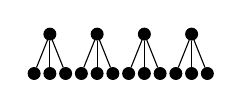
\begin{tikzpicture}
		\tikzset{enclosed/.style={draw, circle, inner sep=0pt, minimum size=.15cm, fill=black}}
		%
		\node[enclosed] (4) at (0.2,0.5) {};
		\node[enclosed] (5) at (0.8,0.5) {};
		\node[enclosed] (6) at (1.4,0.5) {};
		\node[enclosed] (8) at (2,0.5) {};
		
		\node[enclosed] (42) at (0.8,0) {};
		\node[enclosed] (22) at (0.2,0) {};
		\node[enclosed] (21) at (0,0) {};
		\node[enclosed] (23) at (0.4,0) {};
		\node[enclosed] (41) at (0.6,0) {};
		\node[enclosed] (43) at (1,0) {};
		\node[enclosed] (62) at (1.4,0) {};
		\node[enclosed] (82) at (2,0) {};
		\node[enclosed] (81) at (1.8,0) {};
		\node[enclosed] (83) at (2.2,0) {};
		\node[enclosed] (61) at (1.2,0) {};
		\node[enclosed] (63) at (1.6,0) {};
		
		\draw (4) -- (22);
		\draw (4) -- (21);
		\draw (4) -- (23);
		\draw (5) -- (41);
		\draw (5) -- (42);
		\draw (5) -- (43);
		\draw (6) -- (62);
		\draw (6) -- (61);
		\draw (6) -- (63);
		\draw (8) -- (81);
		\draw (8) -- (82);
		\draw (8) -- (83);
	\end{tikzpicture}}}
	\right), \quad \mathcal{G}\left(\vcenter{\hbox{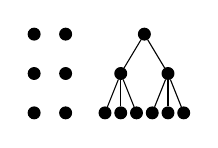
\begin{tikzpicture}
		\tikzset{enclosed/.style={draw, circle, inner sep=0pt, minimum size=.15cm, fill=black}}
		%
		\node[enclosed] (3) at (1.7,1) {};
		\node[enclosed] (6) at (1.4,0.5) {};
		\node[enclosed] (8) at (2,0.5) {};
		
		\node[enclosed] (42) at (0.7,0.5) {};
		\node[enclosed] (22) at (0.3,0.5) {};
		\node[enclosed] (21) at (0.7,1) {};
		\node[enclosed] (23) at (0.3,1) {};
		\node[enclosed] (41) at (0.3,0) {};
		\node[enclosed] (43) at (0.7,0) {};
		\node[enclosed] (62) at (1.4,0) {};
		\node[enclosed] (82) at (2,0) {};
		\node[enclosed] (81) at (1.8,0) {};
		\node[enclosed] (83) at (2.2,0) {};
		\node[enclosed] (61) at (1.2,0) {};
		\node[enclosed] (63) at (1.6,0) {};
		
		\draw (3) -- (6);
		\draw (3) -- (8);
		\draw (6) -- (62);
		\draw (6) -- (61);
		\draw (6) -- (63);
		\draw (8) -- (81);
		\draw (8) -- (82);
		\draw (8) -- (83);
	\end{tikzpicture}}}
	\right), \quad \mathcal{G}\left(\vcenter{\hbox{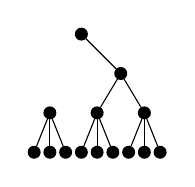
\begin{tikzpicture}
				\tikzset{enclosed/.style={draw, circle, inner sep=0pt, minimum size=.15cm, fill=black}}
				%
				\node[enclosed] (1) at (1.2,1.5) {};
				\node[enclosed] (3) at (1.7,1) {};
				\node[enclosed] (5) at (0.8,0.5) {};
				\node[enclosed] (6) at (1.4,0.5) {};
				\node[enclosed] (8) at (2,0.5) {};
				
				\node[enclosed] (42) at (0.8,0) {};
				\node[enclosed] (41) at (0.6,0) {};
				\node[enclosed] (43) at (1,0) {};
				\node[enclosed] (62) at (1.4,0) {};
				\node[enclosed] (82) at (2,0) {};
				\node[enclosed] (81) at (1.8,0) {};
				\node[enclosed] (83) at (2.2,0) {};
				\node[enclosed] (61) at (1.2,0) {};
				\node[enclosed] (63) at (1.6,0) {};
				
				\draw (1) -- (3);
				\draw (3) -- (6);
				\draw (3) -- (8);
				\draw (5) -- (41);
				\draw (5) -- (42);
				\draw (5) -- (43);
				\draw (6) -- (62);
				\draw (6) -- (61);
				\draw (6) -- (63);
				\draw (8) -- (81);
				\draw (8) -- (82);
				\draw (8) -- (83);
	\end{tikzpicture}}}
	\right), \quad \mathcal{G}\left(\vcenter{\hbox{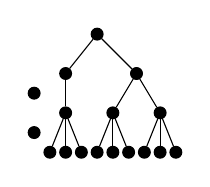
\begin{tikzpicture}
				\tikzset{enclosed/.style={draw, circle, inner sep=0pt, minimum size=.15cm, fill=black}}
				%
				\node[enclosed] (1) at (1.2,1.5) {};
				\node[enclosed] (2) at (0.8,1) {};
				\node[enclosed] (3) at (1.7,1) {};
				\node[enclosed] (5) at (0.8,0.5) {};
				\node[enclosed] (6) at (1.4,0.5) {};
				\node[enclosed] (8) at (2,0.5) {};
				
				\node[enclosed] (9) at (0.4,0.25) {};
				\node[enclosed] (0) at (0.4,0.75) {};
				
				\node[enclosed] (42) at (0.8,0) {};
				\node[enclosed] (41) at (0.6,0) {};
				\node[enclosed] (43) at (1,0) {};
				\node[enclosed] (62) at (1.4,0) {};
				\node[enclosed] (82) at (2,0) {};
				\node[enclosed] (81) at (1.8,0) {};
				\node[enclosed] (83) at (2.2,0) {};
				\node[enclosed] (61) at (1.2,0) {};
				\node[enclosed] (63) at (1.6,0) {};
				
				\draw (1) -- (2);
				\draw (2) -- (5);
				\draw (1) -- (3);
				\draw (3) -- (6);
				\draw (3) -- (8);
				\draw (5) -- (41);
				\draw (5) -- (42);
				\draw (5) -- (43);
				\draw (6) -- (62);
				\draw (6) -- (61);
				\draw (6) -- (63);
				\draw (8) -- (81);
				\draw (8) -- (82);
				\draw (8) -- (83);
	\end{tikzpicture}}}
	\right)
\end{equation*}
before we find the Grundy value of $T_{\{2,2,3\}}$.
\begin{figure}[!ht]
	\centering
	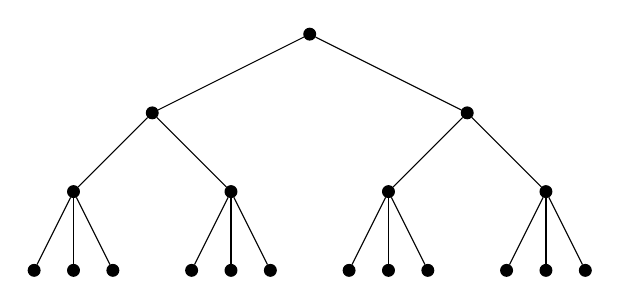
\begin{tikzpicture}
		\tikzset{enclosed/.style={draw, circle, inner sep=0pt, minimum size=.15cm, fill=black}}
		
		\node[enclosed] (1) at (5,4) {};
		\node[enclosed] (2) at (3,3) {};
		\node[enclosed] (3) at (7,3) {};
		\node[enclosed] (4) at (2,2) {};
		\node[enclosed] (5) at (4,2) {};
		\node[enclosed] (6) at (6,2) {};
		\node[enclosed] (8) at (8,2) {};
		\node[enclosed] (42) at (4,1) {};
		\node[enclosed] (22) at (2,1) {};
		\node[enclosed] (21) at (1.5,1) {};
		\node[enclosed] (23) at (2.5,1) {};
		\node[enclosed] (41) at (3.5,1) {};
		\node[enclosed] (43) at (4.5,1) {};
		\node[enclosed] (62) at (6,1) {};
		\node[enclosed] (82) at (8,1) {};
		\node[enclosed] (81) at (7.5,1) {};
		\node[enclosed] (83) at (8.5,1) {};
		\node[enclosed] (61) at (5.5,1) {};
		\node[enclosed] (63) at (6.5,1) {};
		
		\draw (1) -- (2) node[midway, sloped, above] (edge1) {};
		\draw (1) -- (3) node[midway, right] (edge2) {};
		\draw (2) -- (4) node[midway, sloped, above] (edge3) {};
		\draw (2) -- (5) node[midway, sloped, above] (edge4) {};
		\draw (3) -- (6) node[midway, sloped, above] (edge5) {};
		\draw (3) -- (8) node[midway, sloped, above] (edge6) {};
		\draw (4) -- (22) node[midway, sloped, above] (edge7) {};
		\draw (4) -- (21) node[midway, sloped, above] (edge7) {};
		\draw (4) -- (23) node[midway, sloped, above] (edge7) {};
		\draw (5) -- (41) node[midway, sloped, above] (edge7) {};
		\draw (5) -- (42) node[midway, sloped, above] (edge7) {};
		\draw (5) -- (43) node[midway, sloped, above] (edge7) {};
		\draw (6) -- (62) node[midway, sloped, above] (edge7) {};
		\draw (6) -- (61) node[midway, sloped, above] (edge7) {};
		\draw (6) -- (63) node[midway, sloped, above] (edge7) {};
		\draw (8) -- (81) node[midway, sloped, above] (edge7) {};
		\draw (8) -- (82) node[midway, sloped, above] (edge7) {};
		\draw (8) -- (83) node[midway, sloped, above] (edge7) {};
	\end{tikzpicture}
	\caption{$n$-regular tree $T_{\{2,2,3\}}$ \label{fig:ex4}}
\end{figure}

The complexity of this process drastically increases when we try to determine $\mathcal{G}\left(T_{\{a_i\}_{i=0}^{n}}\right)$. Hence, in order to study the Grundy value sequence of the Node-Kayles game on $n$-regular trees in general, we need to adopt another approach.

Despite from it complexity, we can conclude some properties of its Grundy value.
\begin{theorem}
	The Grundy value $\mathcal{G}\left(T_{\{a_i\}_{i=0}^{n}}\right)$ is positive if $a_0$ or $a_1$ is even.
\end{theorem}
\begin{proof}
	If the first player choose to play at root of the graph, the result will be the $a_0\cdot a_1$ copies of the graph $T_{\{a_i\}_{i=2}^{n}}$. If $a_0$ or $a_1$ is even, the Grundy value of this induced subgraph will always be $0$. Therefore, the maximum excluded value of this graph will always be positive.
\end{proof}
\section{Rooted grafting of rooted tree}\label{sec3}
In this section, we investigate the Grundy value associated with Node-Kayles played on the graph construct by connected $2$ $1$-regular tree together by a path. 
\begin{definition}
	Let $G$ and $H$ be a rooted graph and $P_{k}$ be a path of length $k$. The \textit{rooted grafting graph} $G \stackrel{k}{\cdot - \cdot} H$ is construct by identifying a root of graph $G$ to one end of the path $P_{k+1}$ and root of graph $H$ to the other end.
\end{definition}

\begin{figure}[h]
	\centering
		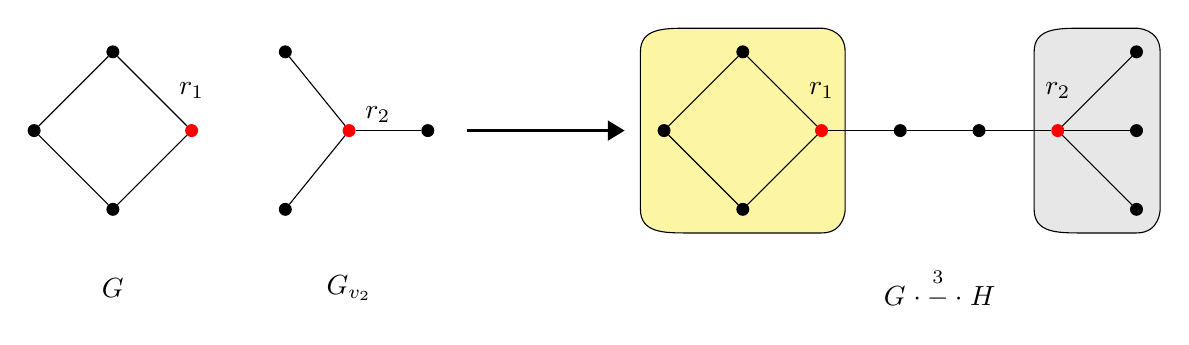
\begin{tikzpicture}
			\tikzset{enclosed/.style={draw, circle, inner sep=0pt, minimum size=.15cm, fill=black}}
			\node[] (1) at (1,-1) {$G$};
			\node[] (2) at (4,-1) {$G_{v_2}$};
			\node[] (3) at (11.5,-1) {$G \stackrel{3}{\cdot - \cdot} H$};
			\draw[-Triangle, very thick](5.5, 1) -- (7.5, 1);
			\node[enclosed] (12) at (0,1) {};
			\node[enclosed] (14) at (1,2) {};
			\node[enclosed] (15) at (1,0) {};
			\node[enclosed, label={above, yshift=.2cm: $r_1$}, color=red] (16) at (2,1) {};
			\draw (12) -- (15);
			\draw (12) -- (14);
			\draw (14) -- (16);
			\draw (16) -- (15);
			
			\node[enclosed, label={right, yshift=.2cm: $r_2$}, color=red] (21) at (4,1) {};
			\node[enclosed] (22) at (5,1) {};
			\node[enclosed] (23) at (3.19,2) {};
			\node[enclosed] (24) at (3.19,0) {};
			\draw (21) -- (22);
			\draw (21) -- (23);
			\draw (21) -- (24);
			\draw  [fill={rgb, 255:red, 248; green, 231; blue, 28 }  ,fill opacity=0.4 ] (7.7,0) .. controls (7.7,-0.3) and (8,-0.3) .. (8.3,-0.3) -- (10,-0.3) .. controls (10.3,-0.3) and (10.3,0) .. (10.3,0) -- (10.3,2) .. controls (10.3,2.3) and (10,2.3) .. (10,2.3) -- (8.3,2.3) .. controls (8,2.3) and (7.7,2.3) .. (7.7,2) -- cycle ;
			
			\draw  [fill={rgb, 255:red, 194; green, 194; blue, 194}  ,fill opacity=0.4 ] (12.7,0) .. controls (12.7,-0.3) and (13,-0.3) .. (13.3,-0.3) -- (14,-0.3) .. controls (14.3,-0.3) and (14.3,0) .. (14.3,0) -- (14.3,2) .. controls (14.3,2.3) and (14,2.3) .. (14,2.3) -- (13.3,2.3) .. controls (13,2.3) and (12.7,2.3) .. (12.7,2) -- cycle ;
			\node[enclosed] (32) at (8,1) {};
			\node[enclosed] (34) at (9,2) {};
			\node[enclosed] (35) at (9,0) {};
			\node[enclosed, label={above, yshift=.2cm: $r_1$}, color=red] (36) at (10,1) {};
			\node[enclosed] (37) at (11,1) {};
			\node[enclosed] (38) at (12,1) {};
			\node[enclosed, label={above, yshift=.2cm: $r_2$}, color=red] (39) at (13,1) {};
			\node[enclosed] (30) at (14,1) {};
			\node[enclosed] (31) at (14,2) {};
			\node[enclosed] (40) at (14,0) {};
			\draw (32) -- (35);
			\draw (32) -- (34);
			\draw (34) -- (36);
			\draw (36) -- (35);
			\draw (36) -- (37);
			\draw (37) -- (38);
			\draw (38) -- (39);
			\draw (39) -- (30);
			\draw (39) -- (31);
			\draw (39) -- (40);
		\end{tikzpicture}
		\caption{The rooted grafting graph $G \stackrel{3}{\cdot - \cdot} H$\label{fig:rootedgrafting}}
\end{figure}
Next, we give the observation to on the rooted grafting graph $T_{\{n\}} \stackrel{k}{\cdot - \cdot}$ for the initial case when $n$ or $k$ is equal to $1$.
\begin{observation}
	$\mathcal{G}\left(T_{\{n\}} \stackrel{1}{\cdot - \cdot}\right) = \mathcal{G}\left(T_{\{n+1\}} \right)$
\end{observation}
\begin{observation}
	$\mathcal{G}\left(T_{\{1\}} \stackrel{k}{\cdot - \cdot}\right) = \mathcal{G}\left(P_{k+2} \right)$
\end{observation}
To determine the Grundy value sequence $\left(\mathcal{G}\left(T_{\{n\}} \stackrel{k}{\cdot - \cdot}\right): n,k \in \mathbb{N}\right)$, we will use the induction to classify the type of the graph.
\begin{theorem}
	For every positive integers $k$ and $n \ge 2$, 
	\begin{align*}
		\mathcal{G}\left(T_{\{n\}} \stackrel{k}{\cdot - \cdot}\right) = \mathcal{G}\left(T_{\{n-2\}} \stackrel{k}{\cdot - \cdot}\right).
	\end{align*}
\end{theorem}
\begin{proof}
	Before we proceed with the induction proof, it is convenient to extend the definitions of $T_{\{n\}} \stackrel{k}{\cdot - \cdot}$ and $P_{k}$ to $-3 \le k \le 1$ and determine the corresponding Grundy values as follows in Table \ref{extendedgrafting}.
	 \begin{table}[]
	 	\centering
	 	\begin{tabular}{|c|c|c|c|cc|}
	 		\hline
	 		\multirow{2}{*}{$k$} & \multirow{2}{*}{$P_k$} & \multirow{2}{*}{$\mathcal{G}\left(P_{k+2} \right)$} & \multirow{2}{*}{$T_{\{n\}} \stackrel{k}{\cdot - \cdot}$} & \multicolumn{2}{c|}{$\mathcal{G}\left(T_{\{n\}} \stackrel{k}{\cdot - \cdot}\right)$}                 \\ \cline{5-6} 
	 		&                       &                          &                    & \multicolumn{1}{c|}{$n$ is odd} & $n$ in even \\ \hline
	 		%$k$  & $P_k$                 & $\mathcal{G}\left(P_{k+2} \right)$ & $T_{\{n\}} \stackrel{k}{\cdot - \cdot}$ & $\mathcal{G}\left(T_{\{n\}} \stackrel{k}{\cdot - \cdot}\right)$ \\ \hline
	 		$-3$ & $\emptyset$  & $0$       & $\cdot \times n-1$  &  \multicolumn{1}{c|}{0} & 1    \\ \hline
	 		$-2$ & $\emptyset$  & $0$       & $\emptyset$  & \multicolumn{1}{c|}{0} & 0     \\ \hline
	 		$-1$ & $\emptyset$  & $0$       & $\cdot \times n$  & \multicolumn{1}{c|}{1} & 0     \\ \hline
	 		$0$  & $\emptyset$  & $0$       & $T_{\{n\}}$  &  \multicolumn{1}{c|}{1} & 2    \\ \hline
	 		$1$  & $\cdot$  	& $1$       & $T_{\{n+1\}}$  & \multicolumn{1}{c|}{2} & 1     \\ \hline
	 	\end{tabular}
	 	\caption{Extended definition of $T_{\{n\}} \stackrel{k}{\cdot - \cdot}$ and $P_{k}$ for $-3 \le k \le 1$. \label{extendedgrafting}}
	 \end{table}
	By definition,
	\begin{align*}
		\mathcal{G}\left(T_{\{n\}} \stackrel{k}{\cdot - \cdot}\right) &= \mathrm{mex}\left(\left\{\mathcal{G}\left(P_{i-2}\right) \oplus \mathcal{G}\left(T_{\{n\}} \stackrel{k-1-i}{\cdot - \cdot}\right) : 1 \le i \le k+2 \right\}\right)\\
		&= \mathrm{mex}\left(\left\{\mathcal{G}\left(P_{i-2}\right) \oplus \mathcal{G}\left(T_{\{n-2\}} \stackrel{k-1-i}{\cdot - \cdot}\right): 1 \le i \le k+2 \right\}\right)\\
		&= \mathcal{G}\left(T_{\{n-2\}} \stackrel{k}{\cdot - \cdot}\right)
	\end{align*}
\end{proof}
\begin{corollary}
	For every positive integer $n,k$,
	\begin{align*}
		\mathcal{G}\left(T_{\{2n-1\}} \stackrel{k}{\cdot - \cdot}\right) = \mathcal{G}\left(T_{\{1\}} \stackrel{k}{\cdot - \cdot}\right) = \mathcal{G}\left(P_{k+2} \right).
	\end{align*}
	and
	\begin{align*}
		\mathcal{G}\left(T_{\{2n\}} \stackrel{k}{\cdot - \cdot}\right) = \mathcal{G}\left(T_{\{2\}} \stackrel{k}{\cdot - \cdot}\right).
	\end{align*}
\end{corollary}

\begin{theorem}\label{thm:t2k}
	The Grundy value sequence $\left(\mathcal{G}\left(T_{\{2\}} \stackrel{k}{\cdot - \cdot}\right) : k \in \mathbb{N}\right)$ is eventually periodic sequence with preperiod lenght $310$ and period $34$.
\end{theorem}
\begin{proof}
	Let $T(k) = \mathcal{G}\left(T_{\{2\}} \stackrel{k}{\cdot - \cdot}\right)$ and $P(k) = \mathcal{G}\left(P_{k}\right)$ be the Grundy value of the game $T_{\{2\}} \stackrel{k}{\cdot - \cdot}$ and $P_k$, respectively.By definition,
	\begin{equation*}
		T(k) = \mathrm{mex}\left(\left\{P(i-2) \oplus T(k-1-i): 1 \le i \le k+2 \right\}\right)
	\end{equation*} 
	With the initial conditions in Table \ref{extendedgrafting}, we can compute the values of sequence $\left(T(k) : 1 \le k \le 441 \right)$, which can be seen in Table \ref{T2k}. The sequence is periodic with period $34$ when $311 \le k \le 441$. Assume that for some $k \ge 442$, $T(i) = T(i-34)$ for all $345 \le i < k$. Then
	\begin{align*}
		T(k) &= \mathrm{mex}\left(\left\{P(i-2) \oplus T(k-1-i): 1 \le i \le k+2 \right\}\right)\\
		&= \mathrm{mex}(\left\{P(i-2) \oplus T(k-1-i): 1 \le i \le k-346 \right\} \\
		&\hspace{1.5cm} \cup \left\{P(i-2) \oplus T(k-1-i): k-345 \le i \le k+2 \right\})\\
		&= \mathrm{mex}(\left\{P(i-2) \oplus T(k-35-i): 1 \le i \le k-346 \right\} \\
		&\hspace{1.5cm} \cup \left\{P(i-36) \oplus T(k-1-i): k-345 \le i \le k+2 \right\})\\
		&= \mathrm{mex}\left(\left\{P(i-2) \oplus T(k-35-i): 1 \le i \le k-32 \right\}\right)\\
		&= T(k-34),
	\end{align*}
	which completes our induction.
	\begin{figure}
		\centering
		\tikzset{every picture/.style={line width=0.75pt}} %set default line width to 0.75pt        
		
		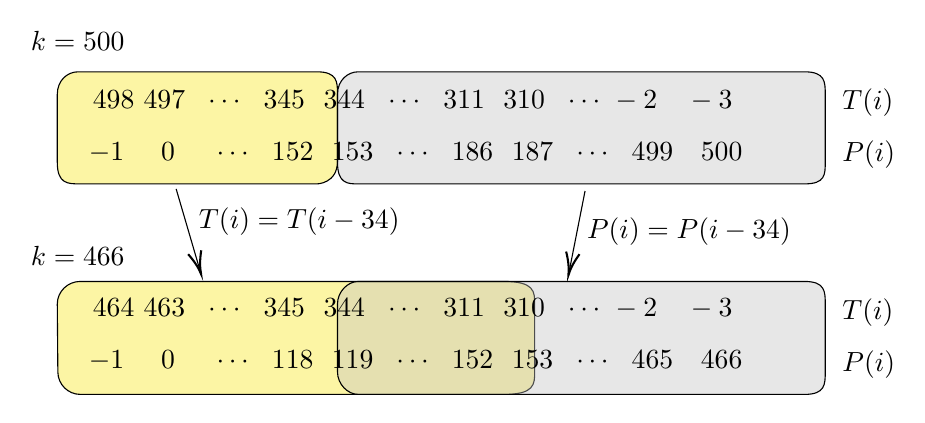
\begin{tikzpicture}[x=0.75pt,y=0.75pt,yscale=-1,xscale=1]
			%uncomment if require: \path (0,300); %set diagram left start at 0, and has height of 300
			
			%Rounded Rect [id:dp25707695535793806] 
			\draw  [fill={rgb, 255:red, 248; green, 231; blue, 28 }  ,fill opacity=0.4 ] (85,87.89) .. controls (85,81) and (90,77) .. (95,77) -- (210,77) .. controls (220,77) and (220,81.87) .. (220,87.89) -- (220,120) .. controls (220,131) and (210,131) .. (210,131) -- (96,131) .. controls (90,131) and (85,131) .. (85,120.54) -- cycle ;
			%Rounded Rect [id:dp37355640029143056] 
			\draw  [fill={rgb, 255:red, 194; green, 194; blue, 194 }  ,fill opacity=0.4 ] (220,87.89) .. controls (220,81) and (225,77) .. (230,77) -- (445,77) .. controls (455,77) and (455,81.87) .. (455,87.89) -- (455,120.54) .. controls (455,126.56) and (455,131) .. (445,131) -- (230,131) .. controls (225,131) and (220,131) .. (220,120.54) -- cycle ;
			
			%Rounded Rect [id:dp9249686119689714] 
			\draw  [fill={rgb, 255:red, 248; green, 231; blue, 28 }  ,fill opacity=0.4 ] (85,188.89) .. controls (85,182.87) and (90,178) .. (96,178) -- (300,178) .. controls (315,178) and (315,182.87) .. (315,188.89) -- (315,221.54) .. controls (315,227.56) and (315,232.43) .. (300,232.43) -- (96.16,232.43) .. controls (90.15,232.43) and (85.27,227.56) .. (85.27,221.54) -- cycle ;
			%Rounded Rect [id:dp8112235307502413] 
			\draw  [fill={rgb, 255:red, 194; green, 194; blue, 194 }  ,fill opacity=0.4 ] (220,188.89) .. controls (220,182.87) and (225,178) .. (230,178) -- (445,178) .. controls (455,178) and (455,182.87) .. (455,188.89) -- (455,221.54) .. controls (455,227.56) and (455,232.43) .. (445,232.43) -- (230,232.43) .. controls (225,232.43) and (220,227.56) .. (220,221.54) -- cycle ;
			
			%Straight Lines [id:da965057370909005] 
			\draw    (142.27,133.43) -- (153.71,172.51) ;
			\draw [shift={(154.27,174.43)}, rotate = 253.69] [color={rgb, 255:red, 0; green, 0; blue, 0 }  ][line width=0.75]    (10.93,-3.29) .. controls (6.95,-1.4) and (3.31,-0.3) .. (0,0) .. controls (3.31,0.3) and (6.95,1.4) .. (10.93,3.29)   ;
			%Straight Lines [id:da39918184970711434] 
			\draw    (339.27,134.43) -- (331.66,173) ;
			\draw [shift={(331.27,174.96)}, rotate = 281.17] [color={rgb, 255:red, 0; green, 0; blue, 0 }  ][line width=0.75]    (10.93,-3.29) .. controls (6.95,-1.4) and (3.31,-0.3) .. (0,0) .. controls (3.31,0.3) and (6.95,1.4) .. (10.93,3.29)   ;
			
			% Text Node
			\draw (71,160) node [anchor=north west][inner sep=0.75pt]   [align=left] {$k=466$};
			% Text Node
			\draw (92,185) node [anchor=north west][inner sep=0.75pt]   [align=left] {$\ \ 464 \ 463 \ \ \cdots \ \ 345 \ \ 344 \ \ \cdots \ \ 311 \ \ 310 \ \ \cdots \ -2 \ \ \ -3$};
			% Text Node
			\draw (99,210) node [anchor=north west][inner sep=0.75pt]   [align=left] {$-1 \ \ \ \ 0 \ \ \ \ \cdots \ \ 118 \ \ 119 \ \ \cdots \ \ 152 \ \ 153 \ \ \cdots \ \ 465 \ \ \ 466$};
			% Text Node
			\draw (462,185) node [anchor=north west][inner sep=0.75pt]   [align=left] {$T(i)$};
			% Text Node
			\draw (462,210) node [anchor=north west][inner sep=0.75pt]   [align=left] {$P(i)$};
			% Text Node
			\draw (71,56) node [anchor=north west][inner sep=0.75pt]   [align=left] {$k=500$};
			% Text Node
			\draw (92,85) node [anchor=north west][inner sep=0.75pt]   [align=left] {$\ \ 498 \ 497 \ \ \cdots \ \ 345 \ \ 344 \ \ \cdots \ \ 311 \ \ 310 \ \ \cdots \ -2 \ \ \ -3$};
			% Text Node
			\draw (99,110) node [anchor=north west][inner sep=0.75pt]   [align=left] {$-1 \ \ \ \ 0 \ \ \ \ \cdots \ \ 152 \ \ 153 \ \ \cdots \ \ 186 \ \ 187 \ \ \cdots \ \ 499 \ \ \ 500$};
			% Text Node
			\draw (462,84) node [anchor=north west][inner sep=0.75pt]   [align=left] {$T(i)$};
			% Text Node
			\draw (462,109) node [anchor=north west][inner sep=0.75pt]   [align=left] {$P(i)$};
			% Text Node
			\draw (152,141) node [anchor=north west][inner sep=0.75pt]   [align=left] {$T(i) = T(i-34)$};
			% Text Node
			\draw (339,146) node [anchor=north west][inner sep=0.75pt]   [align=left] {$P(i) = P(i-34)$};
		\end{tikzpicture}
		\caption{Proof of Theorem}
	\end{figure}
\end{proof}

\begin{theorem}
	For every positive integers $m,n$, let $a = 2 - \left(m \mod 2\right)$ and $b = 2 - \left(n \mod 2 \right)$; thus $a=1$ if $m$ is odd and $2$ if $m$ is even (similarly for $b$). Then
	\begin{equation*}
		\mathcal{G}\left(T_{\{m\}} \stackrel{k}{\cdot - \cdot} T_{\{n\}}\right) = \mathcal{G}\left(T_{\{a\}} \stackrel{k}{\cdot - \cdot} T_{\{b\}}\right).
	\end{equation*}
\end{theorem}
\begin{proof}
	By definition,
	\begin{align*}
		\mathcal{G}\left(T_{\{m\}} \stackrel{k}{\cdot - \cdot} T_{\{n\}}\right) &= \mathrm{mex}\left(\left\{\mathcal{G}\left(T_{\{m\}} \stackrel{i-4}{\cdot - \cdot}\right) \oplus \mathcal{G}\left(T_{\{n\}} \stackrel{k-i}{\cdot - \cdot}\right) : 1 \le i \le k+3 \right\}\right)\\
		&= \mathrm{mex}\left(\left\{\mathcal{G}\left(T_{\{a\}} \stackrel{i-4}{\cdot - \cdot}\right) \oplus \mathcal{G}\left(T_{\{b\}} \stackrel{k-i}{\cdot - \cdot}\right) : 1 \le i \le k+3 \right\}\right)\\
		&= \mathcal{G}\left(T_{\{a\}} \stackrel{k}{\cdot - \cdot} T_{\{b\}}\right).
	\end{align*}
\end{proof}
\begin{corollary}
	For every positive integers $m,n,k$, 
	\begin{align*}
		\mathcal{G}\left(T_{\{2m-1\}} \stackrel{k}{\cdot - \cdot} T_{\{2n-1\}}\right) &= \mathcal{G}\left(T_{\{1\}} \stackrel{k}{\cdot - \cdot} T_{\{1\}}\right) = \mathcal{G}\left(P_{k+3} \right),\\
		\mathcal{G}\left(T_{\{2m\}} \stackrel{k}{\cdot - \cdot} T_{\{2n-1\}}\right) &= \mathcal{G}\left(T_{\{2\}} \stackrel{k}{\cdot - \cdot} T_{\{1\}}\right) = \mathcal{G}\left(T_{\{2\}} \stackrel{k+1}{\cdot - \cdot} \right)\\
		 \intertext{\hspace{1cm} and}
		\mathcal{G}\left(T_{\{2m\}} \stackrel{k}{\cdot - \cdot} T_{\{2n\}}\right) &= \mathcal{G}\left(T_{\{2\}} \stackrel{k}{\cdot - \cdot} T_{\{2\}}\right).
	\end{align*}
\end{corollary}

\begin{theorem}
	The Grundy value sequence $\left(\mathcal{G}\left(T_{\{2\}} \stackrel{k}{\cdot - \cdot} T_{\{2\}}\right) : k \in \mathbb{N}\right)$ is eventually periodic sequence with preperiod lenght $640$ and period $34$.
\end{theorem}
\begin{proof}
	Let $T(k) = \mathcal{G}\left(T_{\{2\}} \stackrel{k}{\cdot - \cdot}\right)$ and $T_2(k) = \mathcal{G}\left(T_{\{2\}} \stackrel{k}{\cdot - \cdot} T_{\{2\}}\right)$be the Grundy value of the game $\left(T_{\{2\}} \stackrel{k}{\cdot - \cdot}\right)$ and $\left(T_{\{2\}} \stackrel{k}{\cdot - \cdot} T_{\{2\}}\right)$, respectively. By definition,
	\begin{equation*}
		T_2(k) = \mathrm{mex}\left(\left\{T(i-4) \oplus T(k-i): 1 \le i \le k+3 \right\}\right)
	\end{equation*}
	With the initial conditions in Table \ref{extendedgrafting}, we can compute the values of sequence $\left(T_2(k): 1 \le k \le 747 \right)$ which can be seen in Table \ref{T2k2}. The sequence is periodic with period $34$ when $641 \le k \le 747$. From Theorem \ref{thm:t2k}, $T(i) = T(i-34)$ for all $i \ge 345$. Then for $k \ge 748$,
	\begin{align*}
		T_2(k) &= \mathrm{mex}\left(\left\{T(i-4) \oplus T(k-i): 1 \le i \le k+3 \right\}\right)\\
		&= \mathrm{mex}(\left\{T(i-4) \oplus T(k-i): 1 \le i \le k-345 \right\}\\
		&\hspace{1.5cm} \cup \left\{T(i-4) \oplus T(k-i): k-344 \le i \le k+3 \right\})\\
		&= \mathrm{mex}(\left\{T(i-4) \oplus T(k-i-34): 1 \le i \le k-345 \right\}\\
		&\hspace{1.5cm} \cup \left\{T(i-38) \oplus T(k-i): k-344 \le i \le k+3 \right\})\\
		&= \mathrm{mex}\left(\left\{T(i-4) \oplus T(k-i-34): 1 \le i \le k-31 \right\}\right)\\
		&= T_{2}(k-34).
	\end{align*}
	which completes our induction.
	\begin{figure}
		\centering
		\tikzset{every picture/.style={line width=0.75pt}} %set default line width to 0.75pt        
		
		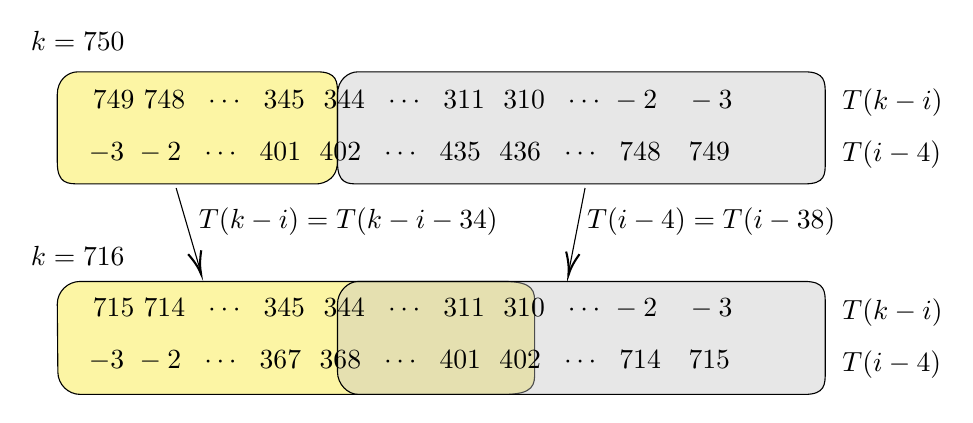
\begin{tikzpicture}[x=0.75pt,y=0.75pt,yscale=-1,xscale=1]
			%uncomment if require: \path (0,300); %set diagram left start at 0, and has height of 300
			
			%Rounded Rect [id:dp25707695535793806] 
			\draw  [fill={rgb, 255:red, 248; green, 231; blue, 28 }  ,fill opacity=0.4 ] (85,87.89) .. controls (85,81) and (90,77) .. (95,77) -- (210,77) .. controls (220,77) and (220,81.87) .. (220,87.89) -- (220,120) .. controls (220,131) and (210,131) .. (210,131) -- (96,131) .. controls (90,131) and (85,131) .. (85,120.54) -- cycle ;
			%Rounded Rect [id:dp37355640029143056] 
			\draw  [fill={rgb, 255:red, 194; green, 194; blue, 194 }  ,fill opacity=0.4 ] (220,87.89) .. controls (220,81) and (225,77) .. (230,77) -- (445,77) .. controls (455,77) and (455,81.87) .. (455,87.89) -- (455,120.54) .. controls (455,126.56) and (455,131) .. (445,131) -- (230,131) .. controls (225,131) and (220,131) .. (220,120.54) -- cycle ;
			
			%Rounded Rect [id:dp9249686119689714] 
			\draw  [fill={rgb, 255:red, 248; green, 231; blue, 28 }  ,fill opacity=0.4 ] (85,188.89) .. controls (85,182.87) and (90,178) .. (96,178) -- (300,178) .. controls (315,178) and (315,182.87) .. (315,188.89) -- (315,221.54) .. controls (315,227.56) and (315,232.43) .. (300,232.43) -- (96.16,232.43) .. controls (90.15,232.43) and (85.27,227.56) .. (85.27,221.54) -- cycle ;
			%Rounded Rect [id:dp8112235307502413] 
			\draw  [fill={rgb, 255:red, 194; green, 194; blue, 194 }  ,fill opacity=0.4 ] (220,188.89) .. controls (220,182.87) and (225,178) .. (230,178) -- (445,178) .. controls (455,178) and (455,182.87) .. (455,188.89) -- (455,221.54) .. controls (455,227.56) and (455,232.43) .. (445,232.43) -- (230,232.43) .. controls (225,232.43) and (220,227.56) .. (220,221.54) -- cycle ;
			
			%Straight Lines [id:da965057370909005] 
			\draw    (142.27,133) -- (153.71,172) ;
			\draw [shift={(154.27,174.43)}, rotate = 253.69] [color={rgb, 255:red, 0; green, 0; blue, 0 }  ][line width=0.75]    (10.93,-3.29) .. controls (6.95,-1.4) and (3.31,-0.3) .. (0,0) .. controls (3.31,0.3) and (6.95,1.4) .. (10.93,3.29)   ;
			%Straight Lines [id:da39918184970711434] 
			\draw    (339.27,133) -- (331.66,172) ;
			\draw [shift={(331.27,174.96)}, rotate = 281.17] [color={rgb, 255:red, 0; green, 0; blue, 0 }  ][line width=0.75]    (10.93,-3.29) .. controls (6.95,-1.4) and (3.31,-0.3) .. (0,0) .. controls (3.31,0.3) and (6.95,1.4) .. (10.93,3.29)   ;
			
			% Text Node
			\draw (71,160) node [anchor=north west][inner sep=0.75pt]   [align=left] {$k=716$};
			% Text Node
			\draw (92,185) node [anchor=north west][inner sep=0.75pt]   [align=left] {$\ \ 715 \ 714 \ \ \cdots \ \ 345 \ \ 344 \ \ \cdots \ \ 311 \ \ 310 \ \ \cdots \ -2 \ \ \ -3$};
			% Text Node
			\draw (99,210) node [anchor=north west][inner sep=0.75pt]   [align=left] {$-3 \ -2 \ \ \cdots \ \ 367 \ \ 368 \ \ \cdots \ \ 401 \ \ 402 \ \ \cdots \ \ 714 \ \ \ 715$};
			% Text Node
			\draw (462,185) node [anchor=north west][inner sep=0.75pt]   [align=left] {$T(k-i)$};
			% Text Node
			\draw (462,210) node [anchor=north west][inner sep=0.75pt]   [align=left] {$T(i-4)$};
			% Text Node
			\draw (71,56) node [anchor=north west][inner sep=0.75pt]   [align=left] {$k=750$};
			% Text Node
			\draw (92,85) node [anchor=north west][inner sep=0.75pt]   [align=left] {$\ \ 749 \ 748 \ \ \cdots \ \ 345 \ \ 344 \ \ \cdots \ \ 311 \ \ 310 \ \ \cdots \ -2 \ \ \ -3$};
			% Text Node
			\draw (99,110) node [anchor=north west][inner sep=0.75pt]   [align=left] {$-3 \ -2 \ \ \cdots \ \ 401 \ \ 402 \ \ \cdots \ \ 435 \ \ 436 \ \ \cdots \ \ 748 \ \ \ 749$};
			% Text Node
			\draw (462,84) node [anchor=north west][inner sep=0.75pt]   [align=left] {$T(k-i)$};
			% Text Node
			\draw (462,109) node [anchor=north west][inner sep=0.75pt]   [align=left] {$T(i-4)$};
			% Text Node
			\draw (152,141) node [anchor=north west][inner sep=0.75pt]   [align=left] {$T(k-i) = T(k-i-34)$};
			% Text Node
			\draw (339,141) node [anchor=north west][inner sep=0.75pt]   [align=left] {$T(i-4) = T(i-38)$};
		\end{tikzpicture}
		\caption{Proof of Theorem}
	\end{figure}
\end{proof}
\section*{Acknowledgement} 
Write support, acknowledgment, dedicatory, and grants here.

%\section*{References} 
\bibliographystyle{abbrv} % We choose the "plain" reference style
\bibliography{refs} % Entries are in the refs.bib file

\begin{landscape}
	\begin{table}[]
		\centering
		\resizebox{20cm}{!}{
		\begin{tabular}{c|cccccccccccccccccccccccccccccccccc}
			& 0 & 1 & 2 & 3 & 4 & 5 & 6 & 7 & 8 & 9 & 10 & 11 & 12 & 13 & 14 & 15 & 16 & 17         & 18 & 19 & 20 & 21 & 22 & 23 & 24 & 25 & 26 & 27 & 28 & 29 & 30 & 31 & 32 & 33 \\ \hline
			0  & 0 & 1 & 1 & 2 & 0 & 3 & 1 & 1 & 0 & 3 & 3  & 2  & 2  & 4  & 0  & 5  & 2  & 2          & 3  & 3  & 0  & 1  & 1  & 3  & 0  & 2  & 1  & 1  & 0  & 4  & 5  & 2  & 7  & 4  \\
			1  & 0 & 1 & 1 & 2 & 0 & 3 & 1 & 1 & 0 & 3 & 3  & 2  & 2  & 4  & 4  & 5  & 5  & \boxed{\textbf{2}} & 3  & 3  & 0  & 1  & 1  & 3  & 0  & 2  & 1  & 1  & 0  & 4  & 5  & 3  & 7  & 4  \\
			2  & 8 & 1 & 1 & 2 & 0 & 3 & 1 & 1 & 0 & 3 & 3  & 2  & 2  & 4  & 4  & 5  & 5  & 9          & 3  & 3  & 0  & 1  & 1  & 3  & 0  & 2  & 1  & 1  & 0  & 4  & 5  & 3  & 7  & 4  \\
			3  & 8 & 1 & 1 & 2 & 0 & 3 & 1 & 1 & 0 & 3 & 3  & 2  & 2  & 4  & 4  & 5  & 5  & 9          & 3  & 3  & 0  & 1  & 1  & 3  & 0  & 2  & 1  & 1  & 0  & 4  & 5  & 3  & 7  & 4  \\
			4  & 8 & 1 & 1 & 2 & 0 & 3 & 1 & 1 & 0 & 3 & 3  & 2  & 2  & 4  & 4  & 5  & 5  & 9          & 3  & 3  & 0  & 1  & 1  & 3  & 0  & 2  & 1  & 1  & 0  & 4  & 5  & 3  & 7  & 4  \\
			5  & 8 & 1 & 1 & 2 & 0 & 3 & 1 & 1 & 0 & 3 & 3  & 2  & 2  & 4  & 4  & 5  & 5  & 9          & 3  & 3  & 0  & 1  & 1  & 3  & 0  & 2  & 1  & 1  & 0  & 4  & 5  & 3  & 7  & 4  \\
			6  & 8 & 1 & 1 & 2 & 0 & 3 & 1 & 1 & 0 & 3 & 3  & 2  & 2  & 4  & 4  & 5  & 5  & 9          & 3  & 3  & 0  & 1  & 1  & 3  & 0  & 2  & 1  & 1  & 0  & 4  & 5  & 3  & 7  & 4  \\
			7  & 8 & 1 & 1 & 2 & 0 & 3 & 1 & 1 & 0 & 3 & 3  & 2  & 2  & 4  & 4  & 5  & 5  & 9          & 3  & 3  & 0  & 1  & 1  & 3  & 0  & 2  & 1  & 1  & 0  & 4  & 5  & 3  & 7  & 4  \\
			8  & 8 & 1 & 1 & 2 & 0 & 3 & 1 & 1 & 0 & 3 & 3  & 2  & 2  & 4  & 4  & 5  & 5  & 9          & 3  & 3  & 0  & 1  & 1  & 3  & 0  & 2  & 1  & 1  & 0  & 4  & 5  & 3  & 7  & 4  \\
			9  & 8 & 1 & 1 & 2 & 0 & 3 & 1 & 1 & 0 & 3 & 3  & 2  & 2  & 4  & 4  & 5  & 5  & 9          & 3  & 3  & 0  & 1  & 1  & 3  & 0  & 2  & 1  & 1  & 0  & 4  & 5  & 3  & 7  & 4  \\
			10 & 8 & 1 & 1 & 2 & 0 & 3 & 1 & 1 & 0 & 3 & 3  & 2  & 2  & 4  & 4  & 5  & 5  & 9          & 3  & 3  & 0  & 1  & 1  & 3  & 0  & 2  & 1  & 1  & 0  & 4  & 5  & 3  & 7  & 4  \\
			11 & 8 & 1 & 1 & 2 & 0 & 3 & 1 & 1 & 0 & 3 & 3  & 2  & 2  & 4  & 4  & 5  & 5  & 9          & 3  & 3  & 0  & 1  & 1  & 3  & 0  & 2  & 1  & 1  & 0  & 4  & 5  & 3  & 7  & 4  \\
			12 & 8 & 1 & 1 & 2 & 0 & 3 & 1 & 1 & 0 & 3 & 3  & 2  & 2  & 4  & 4  & 5  & 5  & 9          & 3  & 3  & 0  & 1  & 1  & 3  & 0  & 2  & 1  & 1  & 0  & 4  & 5  & 3  & 7  & 4 
		\end{tabular}}
		\caption{Grundy value of $P_k$ \label{Pk}}
	\end{table}
	\begin{table}[]
		\centering
		\resizebox{20cm}{!}{
			\begin{tabular}{c|cccccccccccccccccccccccccccccccccc}
				& 0 & 1 & 2 & 3  & 4  & 5 & 6 & 7 & 8 & 9  & 10 & 11 & 12 & 13 & 14 & 15 & 16 & 17 & 18 & 19 & 20 & 21 & 22 & 23 & 24 & 25 & 26 & 27 & 28 & 29 & 30 & 31 & 32 & 33 \\ \hline
				0  & 2 & 1 & 3 & 0  & 0  & 1 & 1 & 4 & 0 & 5  & 1  & 1  & 0  & 0  & 3  & 1  & 2  & 0  & 0  & 1  & 2  & 2  & 3  & 3  & 5  & 2  & 4  & 3  & 3  & 2  & 2  & 1  & 0  & 0  \\
				1  & 2 & 1 & 3 & 0  & 0  & 1 & 7 & 4 & 4 & 6  & 5  & 7  & 0  & 0  & 3  & 1  & 2  & 0  & 0  & 1  & 2  & 2  & 4  & 3  & 5  & 6  & 4  & 7  & 3  & 6  & 2  & 1  & 0  & 0  \\
				2  & 2 & 1 & 3 & 0  & 8  & 1 & 9 & 4 & 2 & 8  & 5  & 9  & 4  & 0  & 3  & 1  & 2  & 0  & 0  & 1  & 2  & 2  & 4  & 8  & 5  & 6  & 4  & 7  & 8  & 6  & 9  & 1  & 0  & 0  \\
				3  & 2 & 1 & 3 & 0  & 8  & 1 & 9 & 4 & 4 & 8  & 5  & 9  & 4  & 0  & 8  & 1  & 2  & 0  & 0  & 1  & 2  & 2  & 4  & 8  & 5  & 9  & 4  & 12 & 8  & 6  & 9  & 9  & 0  & 0  \\
				4  & 2 & 1 & 3 & 0  & 8  & 1 & 9 & 4 & 4 & 14 & 5  & 13 & 4  & 0  & 8  & 1  & 2  & 0  & 0  & 1  & 2  & 2  & 4  & 8  & 5  & 9  & 4  & 12 & 8  & 6  & 9  & 9  & 0  & 0  \\
				5  & 2 & 1 & 3 & 0  & 8  & 1 & 9 & 4 & 4 & 14 & 5  & 13 & 4  & 0  & 8  & 1  & 2  & 4  & 0  & 1  & 2  & 2  & 4  & 8  & 5  & 9  & 4  & 12 & 8  & 6  & 9  & 9  & 0  & 8  \\
				6  & 2 & 9 & 3 & 0  & 8  & 1 & 9 & 4 & 4 & 14 & 5  & 13 & 4  & 0  & 8  & 1  & 2  & 4  & 0  & 1  & 2  & 2  & 4  & 8  & 5  & 9  & 4  & 12 & 8  & 6  & 9  & 9  & 0  & 8  \\
				7  & 2 & 9 & 3 & 0  & 8  & 1 & 9 & 4 & 4 & 14 & 5  & 13 & 4  & 0  & 8  & 1  & 2  & 4  & 0  & 1  & 2  & 2  & 4  & 8  & 5  & 9  & 4  & 12 & 8  & 6  & 9  & 9  & 0  & 8  \\
				8  & 2 & 9 & 3 & 0  & 8  & 1 & 9 & 4 & 4 & 14 & 5  & 13 & 4  & 0  & 8  & 1  & 2  & 4  & 0  & 5  & 2  & 2  & 4  & 8  & 5  & 9  & 4  & 12 & 8  & 6  & 9  & 9  & 0  & 8  \\
				9  & 2 & 9 & 3 & 15 & \boxed{\textbf{8}}  & 1 & 9 & 4 & 4 & 14 & 5  & 13 & 4  & 0  & 8  & 1  & 2  & 4  & 8  & 5  & 13 & 2  & 4  & 8  & 5  & 9  & 4  & 12 & 8  & 6  & 9  & 9  & 0  & 8  \\
				10 & 2 & 9 & 3 & 15 & 14 & 1 & 9 & 4 & 4 & 14 & 5  & 13 & 4  & 0  & 8  & 1  & 2  & 4  & 8  & 5  & 13 & 2  & 4  & 8  & 5  & 9  & 4  & 12 & 8  & 6  & 9  & 9  & 0  & 8  \\
				11 & 2 & 9 & 3 & 15 & 14 & 1 & 9 & 4 & 4 & 14 & 5  & 13 & 4  & 0  & 8  & 1  & 2  & 4  & 8  & 5  & 13 & 2  & 4  & 8  & 5  & 9  & 4  & 12 & 8  & 6  & 9  & 9  & 0  & 8  \\
				12 & 2 & 9 & 3 & 15 & 14 & 1 & 9 & 4 & 4 & 14 & 5  & 13 & 4  & 0  & 8  & 1  & 2  & 4  & 8  & 5  & 13 & 2  & 4  & 8  & 5  & 9  & 4  & 12 & 8  & 6  & 9  & 9  & 0  & 8 
		\end{tabular}}
		\caption{Grundy value of $T_{\{2\}}\stackrel{k}{\cdot - \cdot}$ \label{T2k}}
	\end{table}
	\begin{table}[]
		\centering
		\resizebox{20cm}{!}{
		\begin{tabular}{c|cccccccccccccccccccccccccccccccccc}
			& 0 & 1 & 2 & 3 & 4  & 5 & 6  & 7 & 8  & 9 & 10 & 11 & 12 & 13 & 14 & 15 & 16 & 17 & 18 & 19 & 20 & 21 & 22 & 23 & 24 & 25 & 26 & 27 & 28         & 29 & 30 & 31 & 32 & 33 \\ \hline
			0  & 2 & 1 & 1 & 0 & 2  & 2 & 2  & 3 & 3  & 0 & 1  & 1  & 3  & 0  & 2  & 1  & 1  & 0  & 5  & 5  & 2  & 4  & 4  & 0  & 1  & 1  & 2  & 0  & 3          & 1  & 1  & 0  & 3  & 3  \\
			1  & 2 & 2 & 4 & 3 & 5  & 2 & 2  & 3 & 3  & 0 & 1  & 1  & 3  & 0  & 2  & 1  & 1  & 0  & 6  & 5  & 3  & 4  & 4  & 6  & 1  & 1  & 2  & 0  & 3          & 1  & 1  & 0  & 3  & 3  \\
			2  & 5 & 2 & 4 & 7 & 5  & 6 & 4  & 4 & 8  & 0 & 1  & 1  & 3  & 0  & 2  & 1  & 7  & 0  & 6  & 5  & 3  & 4  & 4  & 6  & 5  & 5  & 2  & 0  & 3          & 1  & 1  & 0  & 8  & 3  \\
			3  & 5 & 4 & 4 & 4 & 5  & 5 & 4  & 4 & 8  & 0 & 6  & 1  & 3  & 0  & 2  & 1  & 7  & 0  & 6  & 5  & 3  & 7  & 4  & 6  & 1  & 5  & 2  & 0  & 3          & 1  & 1  & 0  & 12 & 3  \\
			4  & 5 & 4 & 4 & 7 & 5  & 6 & 4  & 7 & 8  & 0 & 6  & 1  & 3  & 0  & 2  & 1  & 7  & 7  & 6  & 5  & 3  & 4  & 4  & 6  & 5  & 5  & 2  & 0  & 3          & 1  & 1  & 4  & 12 & 3  \\
			5  & 5 & 4 & 4 & 7 & 5  & 6 & 4  & 7 & 8  & 0 & 6  & 1  & 3  & 0  & 2  & 1  & 7  & 7  & 6  & 5  & 3  & 4  & 4  & 6  & 5  & 5  & 2  & 4  & 3          & 5  & 9  & 4  & 12 & 3  \\
			6  & 5 & 6 & 4 & 4 & 5  & 5 & 16 & 7 & 15 & 0 & 6  & 7  & 3  & 8  & 2  & 1  & 7  & 7  & 6  & 11 & 3  & 7  & 4  & 6  & 13 & 5  & 2  & 4  & 3          & 5  & 9  & 4  & 12 & 3  \\
			7  & 5 & 6 & 4 & 4 & 11 & 5 & 16 & 7 & 15 & 6 & 6  & 7  & 3  & 8  & 2  & 14 & 7  & 7  & 6  & 11 & 3  & 7  & 4  & 6  & 13 & 5  & 2  & 4  & 3          & 13 & 9  & 4  & 12 & 3  \\
			8  & 5 & 6 & 4 & 4 & 11 & 5 & 16 & 7 & 15 & 6 & 6  & 7  & 3  & 3  & 2  & 14 & 7  & 7  & 6  & 11 & 3  & 7  & 4  & 6  & 13 & 5  & 2  & 4  & 3          & 13 & 9  & 4  & 4  & 3  \\
			9  & 5 & 6 & 4 & 4 & 11 & 5 & 16 & 7 & 15 & 6 & 6  & 7  & 3  & 3  & 2  & 14 & 7  & 7  & 6  & 11 & 3  & 7  & 4  & 6  & 13 & 5  & 2  & 4  & 3          & 13 & 9  & 4  & 4  & 3  \\
			10 & 5 & 6 & 4 & 4 & 11 & 5 & 16 & 7 & 15 & 6 & 6  & 7  & 3  & 3  & 2  & 14 & 7  & 7  & 6  & 11 & 3  & 7  & 4  & 6  & 13 & 5  & 2  & 4  & 3          & 13 & 9  & 4  & 4  & 3  \\
			11 & 5 & 6 & 4 & 4 & 11 & 5 & 16 & 7 & 15 & 6 & 6  & 9  & 3  & 3  & 2  & 2  & 15 & 7  & 12 & 14 & 3  & 7  & 4  & 6  & 13 & 5  & 2  & 4  & 3          & 13 & 9  & 4  & 4  & 3  \\
			12 & 5 & 6 & 4 & 4 & 11 & 5 & 16 & 7 & 15 & 6 & 6  & 9  & 3  & 3  & 2  & 2  & 15 & 7  & 12 & 14 & 3  & 15 & 4  & 6  & 13 & 5  & 2  & 4  & 3          & 13 & 9  & 4  & 4  & 3  \\
			13 & 5 & 6 & 4 & 4 & 11 & 5 & 16 & 7 & 15 & 6 & 6  & 9  & 3  & 3  & 2  & 2  & 15 & 7  & 12 & 14 & 3  & 15 & 4  & 6  & 13 & 5  & 2  & 4  & 3          & 13 & 9  & 4  & 4  & 14 \\
			14 & 5 & 6 & 4 & 4 & 11 & 5 & 16 & 7 & 15 & 6 & 6  & 9  & 3  & 3  & 2  & 2  & 15 & 7  & 12 & 14 & 3  & 15 & 4  & 6  & 13 & 5  & 2  & 4  & 3          & 13 & 9  & 4  & 4  & 14 \\
			15 & 5 & 6 & 4 & 4 & 11 & 5 & 16 & 7 & 15 & 6 & 6  & 9  & 3  & 3  & 2  & 2  & 15 & 7  & 12 & 14 & 3  & 15 & 4  & 6  & 13 & 5  & 2  & 4  & 3          & 13 & 9  & 4  & 4  & 14 \\
			16 & 5 & 6 & 4 & 4 & 11 & 5 & 16 & 7 & 15 & 6 & 6  & 9  & 3  & 3  & 2  & 2  & 15 & 7  & 12 & 14 & 3  & 15 & 4  & 6  & 13 & 5  & 2  & 4  & 3          & 13 & 9  & 4  & 4  & 14 \\
			17 & 5 & 6 & 4 & 4 & 11 & 5 & 16 & 7 & 15 & 6 & 6  & 9  & 3  & 3  & 2  & 2  & 15 & 7  & 12 & 14 & 3  & 15 & 4  & 6  & 13 & 5  & 2  & 4  & 3          & 13 & 9  & 4  & 4  & 14 \\
			18 & 5 & 6 & 4 & 4 & 11 & 5 & 16 & 7 & 15 & 6 & 6  & 9  & 3  & 3  & 2  & 2  & 15 & 7  & 12 & 14 & 3  & 15 & 4  & 6  & 13 & 5  & 2  & 4  & \boxed{\textbf{3}} & 13 & 9  & 4  & 4  & 14 \\
			19 & 5 & 6 & 4 & 4 & 11 & 5 & 16 & 7 & 15 & 6 & 6  & 9  & 3  & 3  & 2  & 2  & 15 & 7  & 12 & 14 & 3  & 15 & 4  & 6  & 13 & 5  & 2  & 4  & 8          & 13 & 9  & 4  & 4  & 14 \\
			20 & 5 & 6 & 4 & 4 & 11 & 5 & 16 & 7 & 15 & 6 & 6  & 9  & 3  & 3  & 2  & 2  & 15 & 7  & 12 & 14 & 3  & 15 & 4  & 6  & 13 & 5  & 2  & 4  & 8          & 13 & 9  & 4  & 4  & 14 \\
			21 & 5 & 6 & 4 & 4 & 11 & 5 & 16 & 7 & 15 & 6 & 6  & 9  & 3  & 3  & 2  & 2  & 15 & 7  & 12 & 14 & 3  & 15 & 4  & 6  & 13 & 5  & 2  & 4  & 8          & 13 & 9  & 4  & 4  & 14
		\end{tabular}}
		\caption{Grundy value of $T_{\{2\}}\stackrel{k}{\cdot - \cdot} T_{\{2\}}$ \label{T2k2}}
	\end{table}

%	\begin{table}[]
%		\centering
%		\resizebox{20cm}{!}{
%			\begin{tabular}{c|cccccccccccccccccccccccccccccccccc}
%				& 0 & 1 & 2  & 3          & 4 & 5 & 6 & 7 & 8  & 9 & 10 & 11 & 12 & 13 & 14 & 15 & 16 & 17 & 18 & 19 & 20 & 21 & 22 & 23 & 24 & 25 & 26 & 27 & 28 & 29 & 30 & 31 & 32 & 33 \\ \hline
%				0  & 1 & 3 & 0  & 0          & 1 & 1 & 4 & 0 & 5  & 1 & 1  & 0  & 0  & 3  & 1  & 2  & 0  & 0  & 1  & 2  & 2  & 3  & 3  & 5  & 2  & 4  & 3  & 3  & 2  & 2  & 1  & 0  & 0  & 2  \\
%				1  & 1 & 3 & 0  & 0          & 1 & 7 & 4 & 4 & 6  & 5 & 7  & 0  & 0  & 3  & 1  & 2  & 0  & 0  & 1  & 2  & 2  & 4  & 3  & 5  & 6  & 4  & 7  & 3  & 6  & 2  & 1  & 0  & 0  & 2  \\
%				2  & 1 & 3 & 0  & 8          & 1 & 9 & 4 & 2 & 8  & 5 & 9  & 4  & 0  & 3  & 1  & 2  & 0  & 0  & 1  & 2  & 2  & 4  & 8  & 5  & 6  & 4  & 7  & 8  & 6  & 9  & 1  & 0  & 0  & 2  \\
%				3  & 1 & 3 & 0  & 8          & 1 & 9 & 4 & 4 & 8  & 5 & 9  & 4  & 0  & 8  & 1  & 2  & 0  & 0  & 1  & 2  & 2  & 4  & 8  & 5  & 9  & 4  & 12 & 8  & 6  & 9  & 9  & 0  & 0  & 2  \\
%				4  & 1 & 3 & 0  & 8          & 1 & 9 & 4 & 4 & 14 & 5 & 13 & 4  & 0  & 8  & 1  & 2  & 0  & 0  & 1  & 2  & 2  & 4  & 8  & 5  & 9  & 4  & 12 & 8  & 6  & 9  & 9  & 0  & 0  & 2  \\
%				5  & 1 & 3 & 0  & 8          & 1 & 9 & 4 & 4 & 14 & 5 & 13 & 4  & 0  & 8  & 1  & 2  & 4  & 0  & 1  & 2  & 2  & 4  & 8  & 5  & 9  & 4  & 12 & 8  & 6  & 9  & 9  & 0  & 8  & 2  \\
%				6  & 9 & 3 & 0  & 8          & 1 & 9 & 4 & 4 & 14 & 5 & 13 & 4  & 0  & 8  & 1  & 2  & 4  & 0  & 1  & 2  & 2  & 4  & 8  & 5  & 9  & 4  & 12 & 8  & 6  & 9  & 9  & 0  & 8  & 2  \\
%				7  & 9 & 3 & 0  & 8          & 1 & 9 & 4 & 4 & 14 & 5 & 13 & 4  & 0  & 8  & 1  & 2  & 4  & 0  & 1  & 2  & 2  & 4  & 8  & 5  & 9  & 4  & 12 & 8  & 6  & 9  & 9  & 0  & 8  & 2  \\
%				8  & 9 & 3 & 0  & 8          & 1 & 9 & 4 & 4 & 14 & 5 & 13 & 4  & 0  & 8  & 1  & 2  & 4  & 0  & 5  & 2  & 2  & 4  & 8  & 5  & 9  & 4  & 12 & 8  & 6  & 9  & 9  & 0  & 8  & 2  \\
%				9  & 9 & 3 & 15 & \textbf{8} & 1 & 9 & 4 & 4 & 14 & 5 & 13 & 4  & 0  & 8  & 1  & 2  & 4  & 8  & 5  & 13 & 2  & 4  & 8  & 5  & 9  & 4  & 12 & 8  & 6  & 9  & 9  & 0  & 8  & 2  \\
%				10 & 9 & 3 & 15 & 14         & 1 & 9 & 4 & 4 & 14 & 5 & 13 & 4  & 0  & 8  & 1  & 2  & 4  & 8  & 5  & 13 & 2  & 4  & 8  & 5  & 9  & 4  & 12 & 8  & 6  & 9  & 9  & 0  & 8  & 2  \\
%				11 & 9 & 3 & 15 & 14         & 1 & 9 & 4 & 4 & 14 & 5 & 13 & 4  & 0  & 8  & 1  & 2  & 4  & 8  & 5  & 13 & 2  & 4  & 8  & 5  & 9  & 4  & 12 & 8  & 6  & 9  & 9  & 0  & 8  & 2  \\
%				12 & 9 & 3 & 15 & 14         & 1 & 9 & 4 & 4 & 14 & 5 & 13 & 4  & 0  & 8  & 1  & 2  & 4  & 8  & 5  & 13 & 2  & 4  & 8  & 5  & 9  & 4  & 12 & 8  & 6  & 9  & 9  & 0  & 8  & 2 
%		\end{tabular}}
%		\caption{Grundy-value of $T_{2n}\stackrel{k}{\cdot - \cdot}T_{2n+1}$}
%	\end{table}
\end{landscape}

\end{document}

%%
%% End of file `ecrc-template.tex'. 
